\documentclass[addpoints,11pt]{exam}

\usepackage{alltt}
\usepackage[margin=1in]{geometry}   % set up margins
\usepackage[T1]{fontenc}
\usepackage[usenames,dvipsnames]{xcolor}
\usepackage{enumerate}              % fancy enumerate
\usepackage{amsmath}                % used for \eqref{} in this document
\usepackage{amsthm}
\theoremstyle{definition}
\newtheorem{exmp}{Example}[section]
\usepackage{verbatim}               % useful for \begin{comment} and \end{comment}
\usepackage{eurosym}                % used for euro symbol
\usepackage{caption} 
\usepackage{graphicx}
\graphicspath{{Figures/}}
\usepackage{subcaption}
\usepackage{color}
\usepackage{float}
\usepackage{amssymb}
\usepackage{MnSymbol,wasysym}
\usepackage[colorlinks=true]{hyperref}
\hypersetup{colorlinks=true, citecolor=ForestGreen, linkcolor=BlueViolet, urlcolor=Magenta}

\usepackage{array}
\newcolumntype{H}{@{}>{\lrbox0}l<{\endlrbox}}


%Solutions or nah
%\printanswers
%\newcommand{\dd}[1]{{\textbf{\textcolor{red}{#1}}}}
%\newcommand{\ddp}[1]{\par {\textcolor{ForestGreen}{#1}}}

\newcommand{\dd}[1]{}  
\newcommand{\ddp}[1]{}

\setlength\parindent{0pt}
\unframedsolutions
\SolutionEmphasis{\color{red}}
\CorrectChoiceEmphasis{\color{red}}
\renewcommand{\choicelabel}{(\alph{choice})}
\newcommand{\blank}[0]{\underline{\hspace{3cm}}}
\pointformat{\bfseries[\thepoints]}
\pointpoints{pt}{pts}
\pointsinrightmargin

\begin{document}
	
	
	\title{\textbf{Exam 1 \dd{\\Solutions}} \\ \vspace{2 mm} {\large ECON 380} \\ \large{Fall 2017} \\ \large{UNC Chapel Hill}}
	\date{}
	\maketitle
	
	\makebox[\textwidth]{Name:\enspace\hrulefill}
	\\
	
	\makebox[\textwidth]{ONYEN:\enspace\hrulefill}
	\\
	
	\makebox[\textwidth]{Honor Code Signature:\enspace\hrulefill}
	\\
	
	\begin{center}
		\fbox{\fbox{\parbox{6in}{\centering
					\underline{Directions:}
					\begin{itemize}
						\item Fill in your name (Last, first) and PID on your scantron.
						\item For multiple choice questions, clearly circle the answer choice which best answers the question and bubble in the corresponding choice on your scantron.
						\item For short answer questions, show all of your work and justify your answers where needed. 
						\item Round answers to the nearest hundredth.
						\item Assume preferences are transitive, complete, monotone, and convex.
						\item Assume that leisure is income normal. 
						\item Points available: 50
						\item Write legibly, write legibly, write legibly!
						\item Good luck! \smiley{}
					\end{itemize}
		}}}
	\end{center}
	
	\newpage
	
	\subsection*{Multiple Choice \textbf{[2 pts each]}}



The supply and demand for workers in Algeria is shown below:

\begin{figure}[H]
	\centering
	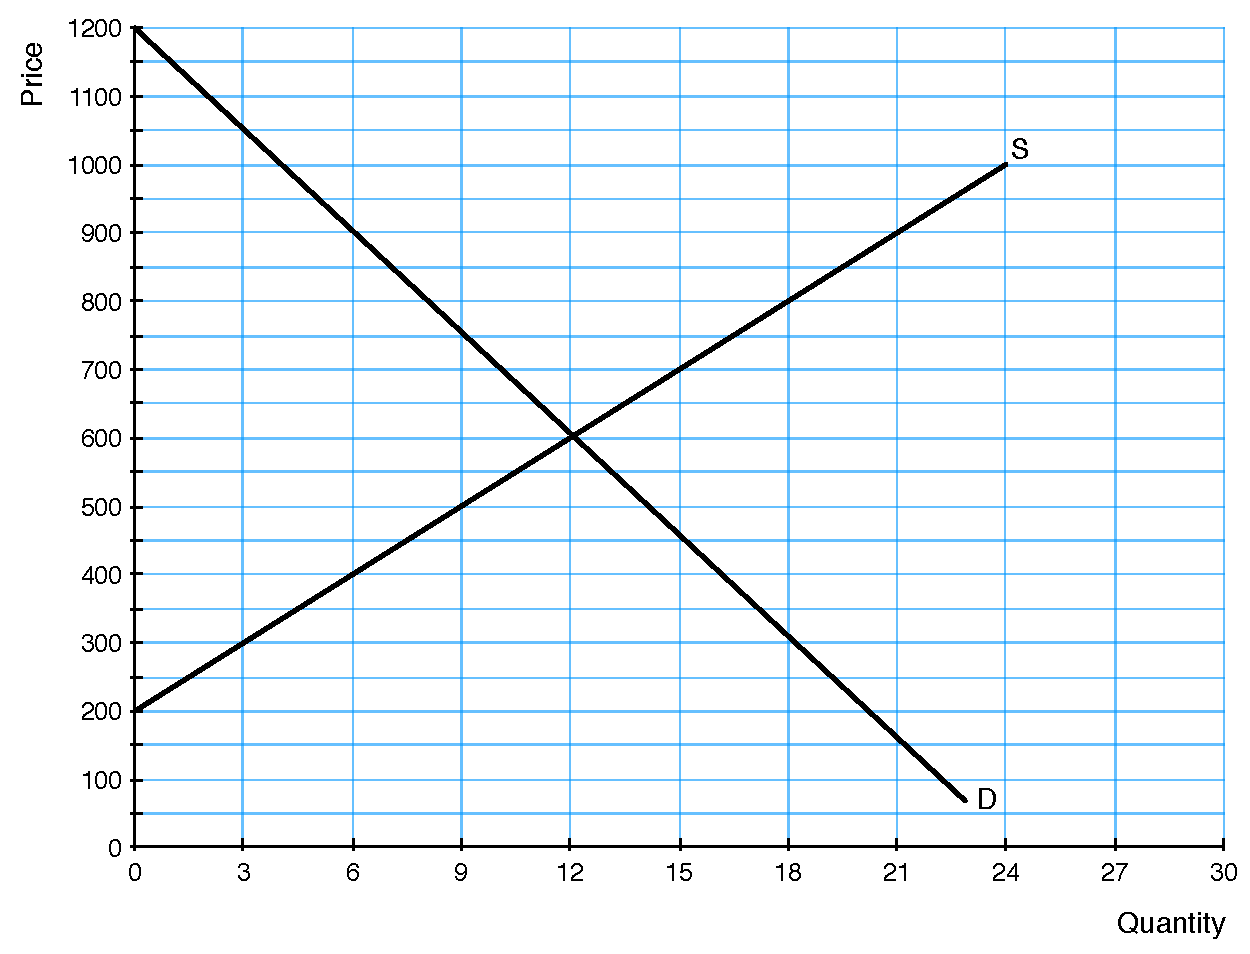
\includegraphics[scale=.45]{Exam1_MC16.pdf}
	\caption{Algerian Labor Market}
\end{figure}


where "quantity" represents the number of workers (in millions) and the "price" is the hourly wage rate in Algerian dinars (DA). Assume this labor market is perfectly competitive.
\\

The government is considering providing firms a wage subsidy of 500 DA per hour for each worker hired which will increase employment to 18 million. Use this information to answer questions \ref{q1}-\ref{q2}: 


\begin{questions}
	
	\question \label{q1} If the government chooses to impose this subsidy, the hourly wage earned by workers will be \blank, while firms will pay \blank per hour out of pocket. 
	
\begin{choices}
	\choice 900 DA; 400 DA
	\choice 300 DA; 800 DA
	\choice 400 DA; 900 DA
	\CorrectChoice 800 DA; 300 DA
	\choice None of the above
\end{choices}

\question If implemented, the deadweight loss of the subsidy would be

\begin{choices}
	\choice 9 billion DA
	\choice 1.5 billion DA
	\choice 3 billion DA
	\choice 4.5 billion DA
	\choice 0 DA.
\end{choices}

\newpage
	
\question \label{q2} How many of the following statements are TRUE?

\begin{enumerate}[i.]
	\item Worker and firm surplus will increase as a result of the subsidy.
	\item The total cost of the subsidy will be lower than the gains to worker and firm surplus.
	\item The subsidy will increase employment relative to the competitive market, but will also increase involuntary unemployment.
\end{enumerate}
	
	
\begin{choices}
	\choice 0
	\CorrectChoice 1
	\choice 2
	\choice 3
\end{choices}
	
 
\question Arias \& Khamis (2008) analyze participation and earnings performances in several sectors in Argentina in order to test whether the labor market is segmented due to ``exclusion'' or comparative advantage considerations. Among which workers did the authors find evidence for the ``exclusion'' story?

\begin{choices}
	\choice Workers engaged in self-employment.
	\choice Workers engaged in home production.
	\CorrectChoice Workers engaged in informal work.
	\choice Workers engaged in any of the above sectors.
	\choice None of the above. The authors did not find evidence for the exclusion story.
\end{choices}

\question All else equal, which of the following correctly describes the relationship between the wage paid to \underline{the last worker} hired in perfectly competitive (PC) labor markets, a labor market with a perfectly discriminating (PD) monopsonist, and a labor market with a non-discriminating (ND) monopsonist?


\begin{choices}
	\choice PC wage = PD monopsonist wage < ND monopsonist wage
	\CorrectChoice PC wage = PD monopsonist wage > ND monopsonist wage
	\choice PC wage > PD monopsonist wage = ND monopsonist wage
	\choice PC wage > PD monopsonist wage = ND monopsonist wage
\end{choices}

\question Abby Lee earns \$30 per hour, regardless of the number of hours she works, and faces a tax rate of 35\% (assume she actually pays). Additionally, she must pay childcare costs of \$10 per hour if she works. Lastly, Abby Lee receives a weekly non-taxed payment of \$200 from her older sister. There are 110 hours in a week for Abby Lee to allocate between work and leisure. If Abby can work 50 weeks each year, which of the following represents the equation for her yearly budget line?

\begin{choices}
	\CorrectChoice $C = 78,750 - 12.50L$
	\choice $C = 68,750 - 12.50L$
	\choice $C = 133,750 - 22.50L$
	\choice $C = 67,750 - 10.50L$
	\choice $C = 78,750 - 12.50L$
\end{choices}

\newpage

\question If discouraged workers become encouraged by recent improvements in the job market and begin searching for jobs, this would cause the unemployment rate to \blank and the labor force participation rate to \blank. 

\begin{choices}
	\choice rise; fall
	\choice fall; rise
	\choice fall; fall
	\CorrectChoice rise; rise
\end{choices}

\question JoJo (aged 17) is graduating from dance school next month. She has received job offers from potential employers, but she cannot start work until after she finishes her program. The BLS would classify JoJo as

\begin{choices}
	\choice unemployed
	\choice employed
	\CorrectChoice out of the labor force
	\choice not in the working population.
\end{choices}

\question Suppose a binding minimum wage is increased. All else equal, in which of the following would the loss in employment be greatest?

\begin{choices}
	\choice A labor market with a relatively elastic supply curve.
	\CorrectChoice A labor market with a relatively elastic demand curve.
	\choice A labor market with a relatively inelastic supply curve.
	\choice A labor market with a relatively inelastic demand curve.
\end{choices}

\question Consider the following bundles of leisure and consumption available to a worker:

\begin{figure}[H]
	\centering
	\includegraphics[scale=.45]{Exam1_MC10}
	\caption{Worker Bundles}
\end{figure}
 
where bundle $B$ lies on the chord connecting bundles $A$ and $C$. If the worker's preferences satisfy the property of convexity, which of the following must be true?

\begin{choices}
	\choice $U(A) > U(B) > U(C)$
	\choice $U(A) > U(B)$ and $U(B) < U(C)$
	\CorrectChoice $U(A) < U(B)$ and $U(B)>U(C)$ 
	\choice $U(A) < U(B) < U(C)$
\end{choices}
	
\end{questions}

\end{document}